% \usepackage[UTF8]{ctex}
% 使用%可以书写注释,在本行内%及以后的内容不会显示在编译后的PDF文件中。

\documentclass[UTF8]{ctexart}

\usepackage{CJKutf8}
\usepackage{geometry}
\usepackage{amsmath}
\usepackage{amssymb}
\usepackage{booktabs}

\usepackage{graphicx}
\usepackage{float}

\usepackage{listings}
\usepackage{color}
\usepackage{xcolor}

\definecolor{ChatGPT}{RGB}{50, 170, 168}
\definecolor{modify}{RGB}{50, 127, 168}

\newcommand{\ch}[1]{\textcolor{ChatGPT}{#1}}
\newcommand{\m}[1]{\textcolor{modify}{#1}}

\definecolor{dkgreen}{rgb}{0,0.6,0}
\definecolor{gray}{rgb}{0.5,0.5,0.5}
\definecolor{mauve}{rgb}{0.58,0,0.82}
\lstset{frame=tb,
        language=Java,
        aboveskip=3mm,
        belowskip=3mm,
        showstringspaces=false,
        columns=flexible,
        basicstyle=\ttfamily\small,
        numbers=none,
        numberstyle=\tiny\color{gray},
        keywordstyle=\color{blue},
        commentstyle=\color{dkgreen},
        stringstyle=\color{mauve},
        breaklines=true,
        breakatwhitespace=true,
        tabsize=3
}
\lstset{frame=tb,
        language=Go,
        aboveskip=3mm,
        belowskip=3mm,
        showstringspaces=false,
        columns=flexible,
        basicstyle = \ttfamily\small,
        numbers=none,
        numberstyle=\tiny\color{gray},
        keywordstyle=\color{blue},
        commentstyle=\color{dkgreen},
        stringstyle=\color{mauve},
        breaklines=true,
        breakatwhitespace=true,
        tabsize=3
}

\usepackage{tikz}
\usetikzlibrary{positioning,shapes,arrows}

\tikzset{
    class/.style={
        rectangle,
        draw=black,
        text centered,
        minimum height=3em
    },
    arrow/.style={
        ->,
        >=stealth,
        thick
    }
}

\usetikzlibrary{shapes.geometric, arrows}

\tikzstyle{startstop} = [rectangle, rounded corners, minimum width=3cm, minimum height=0.8cm,text centered, draw=black, fill=red!30]
\tikzstyle{io} = [trapezium, trapezium left angle=70, trapezium right angle=110, minimum width=3cm, minimum height=0.8cm, text centered, draw=black, fill=blue!30]
\tikzstyle{process} = [rectangle, minimum width=3cm, minimum height=0.8cm, text centered, draw=black, fill=orange!30]
\tikzstyle{decision} = [diamond, minimum width=2cm, minimum height=0.5cm, text centered, draw=black, fill=green!30]
\tikzstyle{arrow} = [thick,->,>=stealth]

% \begin{CJK}{UTF8}{gbsn}
\geometry{a4paper,scale=0.7}
\pagestyle{plain}

    \title{软件设计文档}
    \author{项目名称:升学指导}
    \date{\today}
\begin{document}

    \maketitle

    \begin{center}
        \begin{tabular}{|c|c|}
            \hline
            姓名 & 于海龙 \\	
            \hline
            学号 & 2120220695 \\	
            \hline
            完成作业共花费&72小时\\
            \hline
            ChatGPT 完成任务比例&40\%\\
            \hline
            实现软件功能预计还需要&20天\\
            \hline
        \end{tabular}

        \par
        % 注:文章中加粗标注的内容使用ChatGPT生成。
    \end{center}

    
    % \begin{abstract}
    % \end{abstract}

    \newpage
    \tableofcontents
    \newpage
    
    \section{背景介绍}
    \subsection{升学问题现状}
    \par
    \m{当学生决定进入研究生阶段时需要仔细考虑自己的职业目标、兴趣爱好和能力,以及选择最适合自己的学校、专业和导师}。这项任务存在一些困难,因为存在太多的选择,并且需要考虑非常多不同的因素,例如学校的声誉、专业的难度、导师的研究领域等等。
    
    \par
    当前的学生面临许多的升学问题,这些问题包括了学校选择、专业选择、导师选择等几个方面。作为学生,首先需要确定自己的研究方向,\m{研究方向决定了学生未来的职业发展方向和就业前景};\m{同时学生也会因为选择合适的研究方向更好地发挥自己的优势和兴趣,提高研究效率和成果质量}。学校选择也是一项重要任务,因为\m{学校的排名和声誉可以影响到研究生的就业前景和职业发展};与此同时\m{学校所在地的交通、生活条件等也需要考虑,这些因素可能会影响到研究生的生活质量和学习效果}。

    \subsection{软件开发目标}
    \par
    \m{设计一款升学指导软件的目的是帮助学生更好地规划自己的未来,解决他们在升学过程中所面临的各种问题和挑战}。目前市面上有很多升学指导的软件,\m{如考研帮、留学Go、升学宝和升学通等}。这些市面上的软件具有不同的特色,具体如下:
    
    \begin{enumerate}
        \item 考研帮:\ch{考研帮是一款专门为考研学生提供的软件,它提供了各种考研资讯、历年真题、模拟考试等服务。用户可以通过该软件获取最新的考研政策、报考指南、院校信息等,还可以参加各种在线课程和学习小组,与其他考生交流经验和心得。此外,考研帮还提供了一些实用的工具,如错题本、复习计划、考试倒计时等,帮助学生更好地备考。}
        \item 留学Go:\ch{留学Go是一款为留学生提供服务的软件,它提供了各国留学信息、申请流程、签证办理等方面的指导和建议。用户可以通过该软件了解各国的大学排名、专业设置、学费情况等信息,还可以查看各个大学的官方网站和招生简章,了解具体的申请要求和流程。此外,留学Go还提供了一些实用的功能,如语言测试、文书模板、面试技巧等,帮助学生更好地准备留学申请。}
        \item 升学宝:\ch{升学宝是一款综合性的升学指导软件,它提供了多种服务,包括选校咨询、专业选择、申请指导等。用户可以通过该软件了解各个大学的招生政策、录取标准、课程设置等信息,还可以查看各个专业的就业前景和发展趋势。此外,升学宝还提供了一些实用的功能,如职业测评、志愿填报、面试模拟等,帮助学生更好地规划自己的升学路线。}
        \item 升学通:\ch{升学通是一款为高中生和大学生提供升学指导的软件,它提供了多种服务,包括选科咨询、专业选择、大学排名等。用户可以通过该软件了解各个大学的招生政策、录取标准、课程设置等信息,还可以查看各个专业的就业前景和发展趋势。}
    \end{enumerate}

    \begin{figure}[htp]
        \centering
        \begin{tikzpicture}[node distance=1.8cm]
            \node (student) [class] {学生信息};
            \node (school) [class, below of=student] {学校信息};
            \node (major) [class, below of=school] {专业信息};
            \node (supervisor) [class, below of=major] {导师信息};
            \node (recommendation) [class, right of=school, xshift=3cm] {升学建议};
            \draw [arrow] (student) -- (recommendation);
            \draw [arrow] (school) -- (recommendation);
            \draw [arrow] (major) -- (recommendation);
            \draw [arrow] (supervisor) -- (recommendation);
        \end{tikzpicture}
        \caption{\m{获取升学推荐信息}}
        \label{fig:element}
    \end{figure}

    \par
    这几款软件存在信息来源不够全面、界面设计不简洁直观和功能不全面等问题。因此我们需要为研究生设计一款简单明了的升学指导软件,如图\ref{fig:element}所示。这款软件期待的目标包括:简洁明了的界面设计、完备的数据库设计、高效的匹配算法设计和数据安全设计。\m{一款升学指导软件可以帮助学生更好地选择适合自己的研究生阶段的学校、专业和导师,这对于他们的职业发展和人生规划非常重要,因此这款软件具有很高的实用性和价值}。

    \section{项目概述}

    \subsection{系统功能}
    \par
    该软件的主要功能是为用户提供升学建议,并提供学校、专业和导师的信息查询服务。除此之外,还需要提供用户基本信息管理、学校专业信息管理、后台管理和统计分析的功能。为了可以支持后续的学生培养计划,还可以在未来允许职场性格测试、职业发展分析等功能的接入。

    \subsection{业务描述}

    \subsubsection{用户升学建议查询}

    \par
    用户升学建议查询的主要流程包括:
    \begin{enumerate}
        \item 输入学生信息;包括学习成绩、兴趣爱好、就职意向等,为系统分析数据提供基础支持。
        \item 系统分析数据;根据学生输入的信息和数据库中的学校、专业和导师信息,执行匹配算法和推荐算法,对数据进行分析。
        \item 生成推荐列表;根据上一步分析的结果,使用Top-K策略选择推荐列表,供用户筛选。
        \item 完成选择;用户根据推荐列表完成升学选择。
    \end{enumerate}

    \begin{figure}[htp]
        \centering
        \begin{tikzpicture}[node distance=1.8cm]
          \node (start) [startstop] {开始};
          \node (input) [io, below of=start] {输入学生信息};
          \node (process1) [process, below of=input] {对数据进行分析};
          \node (decision1) [decision, below of=process1, yshift=-0.5cm] {查询相关信息};
          \node (process2a) [process, below of=decision1, yshift=-1cm] {提供学校、专业和导师的信息};
          \node (process2b) [process, below of=process2a, yshift=-0.5cm] {完成选择};
          \node (stop) [startstop, below of=process2b] {结束};
          \draw [arrow] (start) -- (input);
          \draw [arrow] (input) -- (process1);
          \draw [arrow] (process1) -- (decision1);
          \draw [arrow] (decision1) -- node[anchor=east] {yes} (process2a);
          \draw [arrow] (process2a) -- (process2b);
          \draw [arrow] (process2b) -- (stop);
          \draw [arrow] (decision1.west) -- ++(-2,0) |- node[anchor=south] {no} (input.west);
        \end{tikzpicture}
        \caption{\m{输入学生信息查询学校、专业和导师信息流程图}}
        \label{fig:flowchart0}
    \end{figure}
    
    \par
    当用户执行一次升学建议查询时,具体的流程如图\ref{fig:flowchart0}所示。

    \subsubsection{管理员更新学校专业信息}

    \par
    软件管理员更新学校专业和导师信息的主要流程包括:

    \begin{enumerate}
        \item 管理员输入学校信息;用于数据库查询学校信息并执行更新操作。
        \item 管理员输入专业信息;用于数据库查询专业信息并执行更新操作。
        \item 管理员输入导师信息;用于数据库查询导师信息并执行更新操作。
    \end{enumerate}

    \par
    当管理员用户执行一次学校、专业和导师信息更新时,具体的流程如图\ref{fig:flowchart1}所示。

    \begin{figure}[htp]
        \centering
        \begin{tikzpicture}[node distance=1.8cm]
          \node (start) [startstop] {开始};
          \node (input1) [io, below of=start] {输入学校信息};
          \node (process1) [process, below of=input1] {查找学校信息并更新};
          \node (decision1) [decision, below of=process1, yshift=-0.5cm] {专业信息更新?};
          \node (input2) [io, below of=decision1, yshift=-1cm] {输入专业信息};
          \node (process2) [process, below of=input2] {查找专业信息并更新};
          \node (decision2) [decision, below of=process2, yshift=-0.5cm] {导师信息更新?};
          \node (input3) [io, below of=decision2, yshift=-1cm] {输入导师信息};
          \node (process3) [process, below of=input3] {查找并更新导师信息};
          \node (stop) [startstop, below of=process3] {结束};
          \draw [arrow] (start) -- (input1);
          \draw [arrow] (input1) -- (process1);
          \draw [arrow] (process1) -- (decision1);
          \draw [arrow] (decision1.west) -- ++(-2,0) |- node[anchor=south] {no} (input1.west);
          \draw [arrow] (decision1.south) -- node[anchor=west] {yes} (input2.north);
          \draw [arrow] (input2) -- (process2);
          \draw [arrow] (process2) -- (decision2);
          \draw [arrow] (decision2.west) -- ++(-2,0) |- node[anchor=south] {no} (input2.west);
          \draw [arrow] (decision2.south) -- node[anchor=west] {yes} (input3.north);
          \draw [arrow] (input3) -- (process3);
          \draw [arrow] (process3) -- (stop);
        \end{tikzpicture}
        \caption{\m{更新学校和专业信息流程图}}
        \label{fig:flowchart1}
    \end{figure}

    \subsubsection{用户管理}

    \par
    用户注册、登录和登出的主要流程包括:
    \begin{enumerate}
        \item 用户注册;\m{用户需要在注册页面输入用户名、密码、电子邮件地址等信息,并提交注册请求。系统将验证用户输入的信息,如果验证通过,则创建用户账户,并将用户信息保存在用户数据库中。如果验证未通过,则系统将提示用户重新输入信息。}
        \item 用户登录;\m{用户需要在登录页面输入用户名和密码,并提交登录请求。系统将验证用户输入的信息,如果验证通过,则用户登录系统,可以访问系统提供的服务。如果验证未通过,则系统将提示用户重新输入信息。}
        \item 用户注销;\m{用户在登录状态下可以选择注销登录,退出系统。用户注销后,系统将清除用户登录信息,确保用户的账户安全。}    
    \end{enumerate}

    \par
    当用户执行一次账户注册和登录时,具体的流程如图\ref{fig:flowchart2}所示。

    \begin{figure}[htp]
        \centering
        \begin{tikzpicture}[node distance=1.8cm]
          \node (start) [startstop] {开始};
          \node (input1) [io, below of=start] {输入注册信息};
          \node (process1) [process, below of=input1] {创建用户账户};
          \node (input2) [io, below of=process1] {输入账户信息};
          \node (decision1) [decision, below of=input2, yshift=-0.5cm] {用户凭据正确?};
          \node (process2) [process, below of=decision1, yshift=-1cm] {登入};
          \node (decision2) [decision, below of=process2, yshift=-0.5cm] {保持登录?};
          \node (process3) [process, below of=decision2, yshift=-1cm] {登出};
          \node (stop) [startstop, below of=process3] {结束};
          \draw [arrow] (start) -- (input1);
          \draw [arrow] (input1) -- (process1);
          \draw [arrow] (process1) -- (input2);
          \draw [arrow] (input2) -- (decision1);
          \draw [arrow] (decision1.west) -- ++(-2,0) |- node[anchor=south] {no} (input2.west);
          \draw [arrow] (decision1.south) -- node[anchor=west] {yes} (process2);
          \draw [arrow] (process2) -- (decision2);
          \draw [arrow] (decision2.west) -- ++(-2,0) |- node[anchor=south] {no} (input2.west);
          \draw [arrow] (decision2.south) -- node[anchor=west] {yes} (process3);
          \draw [arrow] (process3) -- (stop);
        \end{tikzpicture}
        \caption{\m{用户注册与登录流程图}}
        \label{fig:flowchart2}
    \end{figure}

    \subsubsection{统计分析}
    \par
    管理员执行数据统计分析的主要流程包括:
    \begin{enumerate}
        \item 输入登录信息;\m{管理员需要在登录页面输入用户名和密码,并提交登录请求}。
        \item 验证用户身份;\m{系统将验证管理员输入的信息,如果验证通过,则管理员登录系统,可以访问统计后台数据。如果验证未通过,则系统将提示管理员重新输入信息}。
        \item 访问统计后台数据;\m{管理员登录后,可以访问统计后台数据,并从数据库中检索相关的统计数据。系统将通过管理员账户和数据库来实现这个过程,以保护管理员的隐私和安全,确保管理员可以方便地查看统计数据}。
        \item 生成并输出报告;\m{系统将检索相关的统计数据,并生成报告。报告可以显示统计数据的图表、表格和其他相关信息。生成的报告将输出给管理员。管理员可以查看报告,并根据报告中的统计数据做出正确的决策}。
    \end{enumerate}

    \begin{figure}[htp]
        \centering
        \begin{tikzpicture}[node distance=1.8cm]
          \node (start) [startstop] {开始};
          \node (input1) [io, below of=start] {管理员登录};
          \node (process1) [process, below of=input1] {认证管理员用户信息};
          \node (process2) [process, below of=process1] {链接后端数据库};
          \node (process3) [process, below of=process2] {筛选并聚合数据};
          \node (process4) [process, below of=process3] {生成数据报告};
          \node (output1) [io, below of=process4] {返回报告结果};
          \node (stop) [startstop, below of=output1] {结束};
          \draw [arrow] (start) -- (input1);
          \draw [arrow] (input1) -- (process1);
          \draw [arrow] (process1) -- (process2);
          \draw [arrow] (process2) -- (process3);
          \draw [arrow] (process3) -- (process4);
          \draw [arrow] (process4) -- (output1);
          \draw [arrow] (output1) -- (stop);
        \end{tikzpicture}
        \caption{\m{管理员查看统计数据}}
        \label{fig:flowchart3}
    \end{figure}
    当管理员用户执行一次统计数据查看操作时,主要流程如图\ref{fig:flowchart3}所示。

    \subsection{数据流程描述}
    \subsubsection{数据}
    \par
    在这个软件系统中需要记录保存和管理的数据主要包括:
    \begin{enumerate}
        \item 学生用户信息;学生用户需要提交学生升学相关的数据,包括学生的考试成绩、兴趣爱好、工作目标等内容。除此之外,还需要在数据库中存储用户的凭证信息以供登录使用。
        \item 管理员信息;系统数据库需要存储管理员的凭证信息以供登录使用,并且需要存储管理员的操作记录日志,可以在数据出现问题是及时查找问题并恢复。
        \item 学校信息;系统数据库需要保存学校信息,以供升学建议的生成。
        \item 专业信息;系统数据库需要保存专业信息,专业信息与学校信息关联,以供升学建议的生成。
        \item 导师信息;系统数据库需要保存导师信息,导师信息与学校和专业信息关联,以供升学建议的生成。
    \end{enumerate}
    \subsubsection{数据间的关系}
    \begin{figure}[h!]
        \centering
        \begin{tikzpicture}[node distance=2cm]
          \node (user) [rectangle, draw=black] {用户};
          \node (school) [rectangle, draw=black, below right=2cm and 3cm of user] {学校};
          \node (major) [rectangle, draw=black, below right=2cm and 0.5cm of user] {专业};
          \node (advisor) [rectangle, draw=black, below right=2cm and 0.5cm of school] {导师};
          \node (admin) [rectangle, draw=black, below left=2cm and 0.5cm of school] {管理员};
          \draw [->,>=stealth] (user) -- (major);
          \draw [->,>=stealth] (user) -- (school);
          \draw [->,>=stealth] (user) -- (advisor);
          \draw [->,>=stealth] (school) -- (major);
          \draw [->,>=stealth] (school) -- (advisor);
          \draw [->,>=stealth] (major) -- (advisor);
          \draw [->,>=stealth] (admin) -- (school);
          \draw [->,>=stealth] (admin) -- (advisor);
          \draw [->,>=stealth] (admin) -- (major);
        \end{tikzpicture}
        \caption{存储数据间存在的关系}
        \label{fig:relationship}
    \end{figure}

    \subsection{用户特点}
    \subsubsection{学生用户}
    \par
    \m{学生用户在升学和职业规划方面的需求可能非常复杂和多样化,例如他们可能需要了解不同学校的录取要求、专业课程设置、就业前景等等。学生用户可能对于数据和统计分析方面的内容比较感兴趣,例如各大学专业的录取率、毕业后就业情况等等,这些数据和统计分析可以帮助他们做出更加明智的决策。}
    \par
    \m{虽然现在的学生都很早就开始接触电脑和互联网,但他们的对软件使用娴熟度仍然各不相同。有些学生可能非常熟练地使用计算机和软件,而另一些学生则可能需要花费更多的时间和精力来适应这些技术。除此之外,学生用户通常喜欢有趣、易于理解的界面和互动方式,因此这个软件系统中的学生用户可能会更喜欢具有可视化效果和游戏化设计的界面和体验。}
    \par
    总体而言,需要给学生用户群体提供简单易懂的可视化界面、清晰全面的推荐信息和稳定可靠的系统平台。

    \subsubsection{系统管理员}
    \par
    \m{管理员用户通常是教育机构或学校的教育管理人员,具有一定的教育管理和升学规划方面的专业背景和知识}。管理员用户需要负责升学指导软件系统的管理和运营,因此需要对这些管理员的操作进行明确完整的日志记录。除此之外,同学生用户一样,\m{他们的对软件使用娴熟度也各不相同}。

    \par
    总体而言,需要给管理员用户群体提供简单易懂的可视化界面、稳定可靠的系统平台和完整的日志记录和恢复系统。
    
    \subsection{运行环境要求}
    \subsubsection{前端用户界面}
    \begin{enumerate}
        \item Web 网页前端UI,需要基于Blink内核的类Chrome浏览器、基于WebKit的Safari浏览器、基于Gecko内核的FireFox浏览器和IE浏览器。
        \item Android 移动应用,需要不低于X版本基于 Linux 内核的 Android 操作系统,或不低于X版本的 HarmonyOS 操作系统。
        \item iOS 移动应用,需要不低于X版本的iOS操作系统。
        \item 各种小程序应用,与网页前端UI要求相同,需要基于Blink内核的类Chrome浏览器、基于WebKit的Safari浏览器、基于Gecko内核的FireFox浏览器和IE浏览器。
    \end{enumerate}
    \subsubsection{服务器程序}
    \begin{enumerate}
        \item 网页服务,需要运行在基于 Linux 内核的操作系统,安装 Apache 和 Nginx 服务完成网站部署、反向代理和负载均衡。
        \item 后端服务,需要运行在基于 Linux 内核的操作系统,安装 Java Development Kits 和 Spring Boot 框架。
        \item 容器服务,需要运行在基于 Linux 内核的操作系统,安装 docker 支持容器运行、安装 Kubernetes 进行容器管理。
        \item 消息队列和缓存,需要运行在基于 Linux 内核的操作系统,安装 Kafka 实现数据流分布式管理、安装 RabbitMQ 实现消息队列处理和事务处理、安装 Redis 实现高速缓存、安装 RocketMQ 实现负载均衡和故障转移。
        \item 监控和日志系统,需要监控和日志工具来监控和记录系统的运行状态和性能,以便及时发现和解决问题,\m{常见的监控和日志工具包括Nagios、Zabbix、ELK等}。
    \end{enumerate}
    \subsubsection{数据库}
    \begin{enumerate}
        \item 数据库管理系统,需要安装数据库管理系统(DBMS)管理数据,包括 MySQL 、PostgreSQL 、Oracle 、SQL Server 等。
        \item 数据库连接:需要使用适当的连接方式来连接数据库,常见的连接方式包括 ODB C、JDBC 、ADO.NET等。
        \item 编程语言和框架,需要使用编程语言和框架来编写数据库相关的代码,常见的编程语言和框架包括Java和Spring Boot。
        \item 数据备份与恢复,需要安装自动备份软件,实现物理备份和逻辑备份,使用完全备份、增量备份、热备份和冷备份结合的方法保障数据库数据的安全。
    \end{enumerate}

    \section{基本设计概述}
    \subsection{用户界面}
    \subsubsection{Web前端界面}
    \par
    这个升学指导软件的前端Web系统需要具备以下要求:
    \begin{enumerate}
        \item 用户友好性:前端Web系统需要具备良好的用户界面和用户体验,易于操作和使用,使用户能够轻松地找到所需信息和功能。
        \item 响应式布局:前端Web系统需要具备响应式布局,能够自适应不同的设备和屏幕大小,包括PC端、手机端、平板电脑等,以便用户能够在不同设备上进行访问和使用。
        \item \m{多媒体支持:前端Web系统需要支持多种多媒体格式,包括音频、视频、图片等,以便用户能够获取到更加丰富的信息和资源}。
        \item 数据可视化:前端Web系统需要支持数据可视化,以便用户能够通过图表、表格等方式更加直观地查看和分析数据和统计信息。
        \item \m{安全性和稳定性:前端Web系统需要具备安全性和稳定性,包括对用户数据和隐私的保护、防止恶意攻击、避免系统崩溃等方面的保障,保证用户的使用体验和数据安全}。
        \item \m{SEO优化:前端Web系统需要进行搜索引擎优化,包括网站结构、页面内容、关键词等方面的优化,以便更好地被搜索引擎收录和推荐,提高网站的流量和用户数量}。
        \item \m{可扩展性和可维护性:前端Web系统需要具备可扩展性和可维护性,以便在未来能够根据需要添加新的功能和模块,同时保证代码的可读性和易于维护}。
    \end{enumerate}

    \subsubsection{Android前端界面}
    \m{
    \begin{enumerate}
        \item 用户友好性:Android前端系统需要具备良好的用户界面和用户体验,易于操作和使用,使用户能够轻松地找到所需信息和功能。
        \item 响应式布局:Android前端系统需要具备响应式布局,能够自适应不同的设备和屏幕大小,包括手机、平板电脑等,以便用户能够在不同设备上进行访问和使用。
        \item 多媒体支持:Android前端系统需要支持多种多媒体格式,包括音频、视频、图片等,以便用户能够获取到更加丰富的信息和资源。
        \item 数据可视化:Android前端系统需要支持数据可视化,以便用户能够通过图表、表格等方式更加直观地查看和分析数据和统计信息。
        \item 安全性和稳定性:Android前端系统需要具备安全性和稳定性,包括对用户数据和隐私的保护、防止恶意攻击、避免应用程序崩溃等方面的保障,保证用户的使用体验和数据安全。
        \item 多语言支持:Android前端系统需要支持多语言,以便用户能够选择自己熟悉的语言进行使用。
        \item 可扩展性和可维护性:Android前端系统需要具备可扩展性和可维护性,以便在未来能够根据需要添加新的功能和模块,同时保证代码的可读性和易于维护。
        \item 适配不同操作系统版本:Android前端系统需要适配不同的Android系统版本,以便用户能够在不同版本的Android系统上使用应用程序。
    \end{enumerate}
    }

    \subsubsection{iOS前端界面}
    \m{
        \begin{enumerate}
            \item 用户友好性:iOS前端系统需要具备良好的用户界面和用户体验,易于操作和使用,使用户能够轻松地找到所需信息和功能。
            \item 响应式布局:iOS前端系统需要具备响应式布局,能够自适应不同的设备和屏幕大小,包括iPhone、iPad等,以便用户能够在不同设备上进行访问和使用。
            \item 多媒体支持:iOS前端系统需要支持多种多媒体格式,包括音频、视频、图片等,以便用户能够获取到更加丰富的信息和资源。
            \item 数据可视化:iOS前端系统需要支持数据可视化,以便用户能够通过图表、表格等方式更加直观地查看和分析数据和统计信息。
            \item 安全性和稳定性:iOS前端系统需要具备安全性和稳定性,包括对用户数据和隐私的保护、防止恶意攻击、避免应用程序崩溃等方面的保障,保证用户的使用体验和数据安全。
            \item 多语言支持:iOS前端系统需要支持多语言,以便用户能够选择自己熟悉的语言进行使用。
            \item 可扩展性和可维护性:iOS前端系统需要具备可扩展性和可维护性,以便在未来能够根据需要添加新的功能和模块,同时保证代码的可读性和易于维护。
            \item 适配不同iOS系统版本:iOS前端系统需要适配不同的iOS系统版本,以便用户能够在不同版本的iOS系统上使用应用程序。
            \end{enumerate}
    }

    \subsubsection{小程序前端界面}
    \m{
        \begin{enumerate}
            \item 用户友好性:小程序前端系统需要具备良好的用户界面和用户体验,易于操作和使用,使用户能够轻松地找到所需信息和功能。
            \item 响应式布局:小程序前端系统需要具备响应式布局,能够自适应不同的设备和屏幕大小,包括手机、平板电脑等,以便用户能够在不同设备上进行访问和使用。
            \item 多媒体支持:小程序前端系统需要支持多种多媒体格式,包括音频、视频、图片等,以便用户能够获取到更加丰富的信息和资源。
            \item 数据可视化:小程序前端系统需要支持数据可视化,以便用户能够通过图表、表格等方式更加直观地查看和分析数据和统计信息。
            \item 安全性和稳定性:小程序前端系统需要具备安全性和稳定性,包括对用户数据和隐私的保护、防止恶意攻击、避免应用程序崩溃等方面的保障,保证用户的使用体验和数据安全。
            \item 多语言支持:小程序前端系统需要支持多语言,以便用户能够选择自己熟悉的语言进行使用。
            \item 可扩展性和可维护性:小程序前端系统需要具备可扩展性和可维护性,以便在未来能够根据需要添加新的功能和模块,同时保证代码的可读性和易于维护。
            \item 适配不同小程序平台:小程序前端系统需要适配不同的小程序平台,例如微信小程序、支付宝小程序等,以便用户能够在不同的小程序平台上使用应用程序。
            \end{enumerate}
    }

    \subsection{后端程序设计}
    \subsubsection{网页服务}
    \begin{enumerate}
        \item 可靠性和稳定性:Web服务器需要具备高可靠性和稳定性,以保证系统的稳定运行和数据的安全。
        \item 高并发处理能力:Web服务器需要具备高并发处理能力,能够同时处理大量用户请求和访问,以保证系统的响应速度和性能。
        \item 安全性和防护能力:Web服务器需要具备安全性和防护能力,包括防止恶意攻击、保护用户数据和隐私、防止系统被攻击等方面的保障。
        \item 负载均衡:Web服务器需要支持负载均衡,以便将用户请求和访问均匀地分配到不同的服务器节点上,提高系统的并发能力和性能。
        \item 高可用性:Web服务器需要具备高可用性,包括故障自动切换、容错机制、备份和恢复等方面的保障,以保证系统的连续性和可用性。
        \item CDN加速:Web服务器需要支持CDN加速,以便能够通过CDN分发内容和资源,提高系统的访问速度和性能。
        \item 数据备份和恢复:Web服务器需要支持数据备份和恢复,以保证数据的安全和完整性。
        \item 高效的日志管理:Web服务器需要具备高效的日志管理,能够对系统运行日志进行收集、存储、分析和展示,以便进行系统管理和优化。
        \item 高效的缓存管理:Web服务器需要具备高效的缓存管理,能够对系统的缓存进行管理和优化,提高系统的性能和并发能力。
    \end{enumerate}

    \subsubsection{后端服务}
    \m{
        \begin{enumerate}
            \item 可扩展性和可维护性:后端服务需要具备可扩展性和可维护性,以便在未来能够根据需要添加新的功能和模块,同时保证代码的可读性和易于维护。
            \item 安全性和稳定性性:后端服务需要具备安全性和稳定性,包括对用户数据和隐私的保护、防止恶意攻击、避免应用程序崩溃等方面的保障,保证用户的使用体验和数据安全。
            \item 高并发处理能力:后端服务需要具备高并发处理能力,能够同时处理大量用户请求和访问,以保证系统的响应速度和性能。
            \item 缓存管理:后端服务需要具备缓存管理,能够对数据和资源进行缓存处理,提高系统的响应速度和性能。
            \item 数据库管理:后端服务需要对数据库进行管理,包括数据的存储、查询、更新和删除等操作,以便实现数据的持久化和管理。
            \item RESTful API设计:后端服务需要设计和实现RESTful API接口,以便前端和其他系统能够通过API接口与后端服务进行通信和数据交互。
            \item 消息队列:后端服务需要支持消息队列,以便能够实现异步处理、任务调度和事件驱动等功能。
            \item 日志记录和监控:后端服务需要支持消息队列,以便能够实现异步处理、任务调度和事件驱动等功能。
            \item 安全认证和授权:后端服务需要进行安全认证和授权,以保证系统的安全性和用户数据的安全。
        \end{enumerate}
    }

    \subsubsection{数据库服务}
    \m{
        \begin{enumerate}
            \item 可靠性和稳定性:数据库服务需要具备高可靠性和稳定性,以保证数据的安全和可靠性。
            \item 高性能和高可用性:数据库服务需要具备高性能和高可用性,能够支持大量并发访问和高效的数据处理,同时保证系统的连续性和可用性。
            \item 数据库备份和恢复:数据库服务需要支持数据备份和恢复,以保证数据的安全和完整性。
            \item 数据库性能优化:数据库服务需要进行性能优化,包括索引优化、查询优化、缓存优化等方面的优化,以提高数据库的响应速度和性能。
            \item 数据库安全管理:数据库服务需要进行安全管理,包括用户认证和授权、数据加密、访问控制等方面的管理,以保证数据的安全和隐私。
            \item 数据库监控和管理:数据库服务需要进行监控和管理,包括数据库状态监控、性能分析、容量规划等方面的管理,以保证数据库的稳定性和可用性。
            \item 数据库升级和迁移:数据库服务需要支持数据库升级和迁移,以便能够根据需要进行系统升级和数据迁移。
            \item 数据库备份和恢复策略:数据库服务需要制定数据库备份和恢复策略,包括备份周期、备份方式、备份存储和恢复流程等方面的策略,以保证数据的安全和可靠性。
            \item 数据库容灾和故障恢复:数据库服务需要具备容灾和故障恢复能力,包括故障自动切换、容错机制、备份和恢复等方面的保障,以保证数据的连续性和可用性。
        \end{enumerate}
    }
    
    \subsection{功能需求}
    \subsubsection{升学指导}
    \begin{enumerate}
        \item 业务定义与描述:\ch{该升学软件是一款提供升学辅助服务的应用程序,旨在帮助用户了解各种高等教育课程和学位的信息,包括申请条件、申请过程和入学要求。该应用程序将提供以下功能:学校搜索、课程搜索、申请流程指南、入学要求和申请条件。}
        \item 适用的用户类型,指操作本功能所需的授权:该应用程序面向认证的学生用户,通过学生授权即可使用。
        \item 功能项的主要页面或样式:该应用程序将提供一个网页界面,其中包括学校搜索、课程搜索、申请流程指南、入学要求和申请条件等功能项,用户可以在该网页上进行操作。
        \item 约束条件和特殊考虑:该应用程序不涉及需要计算机化的功能,所有信息都是基于已有的教育机构和课程信息提供的。由于教育机构和课程信息可能会发生变化,因此系统需要定期更新数据以保持准确性。
    \end{enumerate}
    \par
    输入:学校名称、地理位置、学校类型等搜索条件;学生成绩和学生信息,用户的查找优先级设置。
    \par
    输出:\m{学校搜索结果,包括学校名称、地理位置、学校类型、排名等信息;
    申请流程指南,包括申请时间、材料提交、面试安排等信息;
    入学要求,包括学历要求、语言要求、考试要求等信息;
    申请条件,包括申请资格、申请材料、申请费用等信息。}

    \par
    \m{在异常情况下,例如用户输入的搜索条件不符合要求或者搜索结果为空时,系统将会提示用户重新输入或者提供其他相关信息。}

    \subsubsection{后台管理}
    \begin{enumerate}
        \item 业务定义与描述:\m{该升学软件后台管理系统是一款提供升学辅助服务的应用程序,旨在帮助管理员管理学校、专业、导师和申请流程信息。该应用程序将提供以下功能:学校管理、专业管理、导师管理、申请流程管理、用户管理和数据统计。}
        \item 该应用程序面向管理员用户开放,需要授权才能使用。
        \item 功能项的主要页面或样式:该应用程序将提供一个网页界面,其中包括学校管理、专业管理、导师管理、申请流程管理、用户管理和数据统计等功能项,管理员可以在该网页上进行操作。
        \item 约束条件和特殊考虑:\m{该应用程序需要保护用户数据的安全性和隐私,因此需要采用安全措施来防止未经授权的访问。另外,由于学校、专业、导师和申请流程信息可能会发生变化,因此需要及时更新数据库信息,以确保数据的准确性和时效性。同时,需要遵守数据保护和隐私法规,保护用户隐私信息。另外,应用程序需要具有良好的可扩展性和可维护性,以适应未来的需求变化和技术升级。}
    \end{enumerate}
    \par
    输入:学校信息、专业信息、导师信息、申请流程信息、用户信息。
    \par
    输出:学校信息、专业信息、导师信息、申请流程信息、用户信息、统计信息。
    \par
    在异常情况下,例如用户输入的数据格式不正确或者保存失败时,系统将会提示管理员重新输入或者提供其他相关信息。

    \subsection{非功能需求}
    \subsubsection{系统可用性}
    \m{
        \begin{enumerate}
            \item 系统可靠性:系统需要具备高可靠性和稳定性,以确保系统的持续运行和提供可靠的服务。
            \item 用户友好性:系统需要采用用户友好的界面设计和操作流程,以提高用户的使用体验。
            \item 可访问性:系统需要具备可访问性,以支持不同类型的用户(如残障人士)使用系统。
            \item 系统可维护性:系统需要具备可维护性,以方便后续的维护和升级工作。
            \item 系统安全性:系统需要具备高安全性,以保护用户的数据和隐私信息。
            \item 系统可扩展性:系统需要具备可扩展性,以应对未来的业务需求变化和技术升级。
        \end{enumerate}
    }

    \subsubsection{系统性能}
    \m{
        \begin{enumerate}
            \item 响应时间:系统响应用户请求的时间需要尽量短,以提高用户体验。
            \item 吞吐量:系统需要具备处理大量数据的能力,以确保系统的高效性。
            \item 并发处理能力:系统需要具备同时处理多个用户请求的能力,以支持多用户同时访问系统。
            \item 资源利用率:系统需要合理利用资源,如CPU、内存、磁盘等,以确保系统的高效性和稳定性。
            \item 性能测试:系统需要进行全面的性能测试,包括负载测试、压力测试、性能监控等,以评估系统的性能和稳定性。
        \end{enumerate}
    }
    \subsubsection{安全性}
    \par
    \m{该系统需要确保用户数据的安全性和隐私,防止未经授权的访问和数据泄露等问题。系统应采用安全措施,如加密技术、身份验证、访问控制和审计等,以保护用户数据的安全性和隐私。}
    \m{
        \begin{enumerate}
            \item 用户身份验证:为了保证系统的安全性,需要对用户进行身份验证,以确保只有授权用户才能访问系统。可以采用用户名和密码、短信验证码、指纹识别等多种身份验证方式,以增强系统的安全性。
            \item 数据加密:对于敏感数据和隐私信息,需要采用数据加密技术进行保护。可以采用对称加密算法或非对称加密算法对数据进行加密,以确保数据在传输和存储过程中的安全性。
            \item 访问控制:为了保护系统的安全性,需要对用户进行访问控制,以确保只有授权用户才能访问系统的特定功能或数据。可以采用基于角色或基于权限的访问控制机制,以确保系统的安全性。
            \item 审计日志:为了跟踪系统的操作和异常行为,需要记录系统的审计日志。可以记录用户的登录和退出、操作行为、异常事件等信息,以便对系统进行监控和审计。
            \item 异常处理:对于系统的异常情况,需要采取相应的处理措施,以保证系统的安全性。例如,系统出现SQL注入、跨站脚本攻击等安全漏洞时,需要采取相应的修复措施,防止黑客入侵和数据泄露等问题。
            \item 数据备份:为了保证数据的安全性和可靠性,需要对数据进行备份。可以采用定期备份、增量备份等方式,以确保数据在系统故障或数据丢失的情况下能够及时恢复。
        \end{enumerate}
    }
    \subsubsection{可靠性}
    该系统需要保证高可靠性,确保系统运行的稳定性和可用性。系统应具有故障恢复和备份机制,以确保在系统故障或数据丢失的情况下,能够及时恢复系统运行和数据。
    \m{
        \begin{enumerate}
            \item 故障恢复:为了保证系统的可靠性,系统需要具备故障恢复的能力。当系统出现故障时,应能够及时发现并采取相应的措施进行恢复,以保证系统可以正常运行。例如,可以采用备份机制、冗余设计等方式增强系统的故障恢复能力。
            \item 数据备份和恢复:为了保证数据的可靠性和完整性,需要对数据进行备份和恢复。可以采用定期备份、增量备份等方式,以确保数据在系统故障或数据丢失的情况下能够及时恢复。同时,需要测试数据恢复的可行性和正确性,以确保数据能够完全恢复。
            \item 系统监控和报警:为了及时发现系统的异常情况,需要对系统进行监控和报警。可以采用实时监控、日志审计等方式,及时发现系统的异常情况并进行处理。同时,需要设置报警机制,当系统出现异常时,能够及时通知相关人员进行处理,以保证系统的可靠性和稳定性。
            \item 代码质量和测试:为了保证系统的可靠性,需要具备高质量的代码和测试。可以采用代码规范、代码审查等方式,确保代码的可读性、可维护性和可靠性。同时,需要进行全面的测试,包括单元测试、集成测试、系统测试等,以确保系统的功能和性能均符合要求。
            \item 负载均衡:为了保证系统的可靠性和性能,需要采用负载均衡技术,以均衡系统的负载和流量。可以采用硬件负载均衡器或软件负载均衡器,以确保系统的高可用性和稳定性。
            \item 高可用性设计:为了保证系统的可靠性和稳定性,需要采用高可用性设计。可以采用冗余设计、灾备设计等方式,以确保系统在出现故障时能够自动切换到备份系统,保证系统的可用性和稳定性。
            \item 容错性和可恢复性:为了保证系统的可靠性和容错性,需要采用容错和可恢复性设计。可以采用异常处理机制、事务处理机制、数据校验等方式,以确保系统在出现异常情况时能够自动恢复并保证数据的完整性和正确性。
        \end{enumerate}
    }
    \subsubsection{可维护性}
    该系统需要具有良好的可维护性,以保证系统的可持续发展。系统应具有清晰的代码结构、易于维护和扩展的架构设计和完善的文档和注释,以方便后续开发和维护工作。
    
    \m{
        \begin{enumerate}
            \item 可读性和可维护性:为了保证系统的可维护性,需要具备高质量的代码和易于维护的结构。可以采用代码规范、代码注释等方式,提高代码的可读性和可维护性。同时,需要对代码进行优化和重构,以确保代码的可扩展性和可维护性。
            \item 设计模式和架构:为了保证系统的可维护性,需要采用合适的设计模式和架构,以提高系统的可扩展性和可维护性。可以采用MVC、MVP、MVVM等设计模式,以及分层、微服务、SOA等架构模式,以确保系统的可维护性和可扩展性。
            \item 测试和调试:为了保证系统的可维护性,需要进行全面的测试和调试工作。可以采用自动化测试、单元测试、集成测试、系统测试等方式,以及调试工具和技术,以确保系统的稳定性和可维护性。
            \item 文档和知识库:为了保证系统的可维护性,需要建立完善的文档和知识库,以便后续的维护和升级工作。可以建立系统的设计文档、用户手册、API文档等,以及建立知识库和FAQ,以提供后续维护人员使用。
            \item 版本控制和发布管理:为了保证系统的可维护性和升级能力,需要采用合适的版本控制和发布管理机制。可以采用Git、SVN等版本控制工具,以及自动化发布工具和流程,以确保系统的可维护性和升级能力。
            \item 代码审查和重构:为了保证系统的可维护性,需要进行代码审查和重构工作。可以采用代码审查工具和流程,以及重构工具和技术,对系统的代码进行优化和重构,以提高代码的可读性、可维护性和可扩展性。
            \item 合理的技术选型和架构设计:为了保证系统的可维护性,需要采用合理的技术选型和架构设计。可以采用成熟、稳定、易于维护的技术和工具,以及合理的架构设计,以确保系统的可维护性和稳定性。
        \end{enumerate}
    }
    
    \subsubsection{可扩展性}
    该系统需要具有良好的可扩展性,以应对未来的业务需求变化和技术升级。系统应具有模块化的架构设计、可插拔的功能组件和灵活的配置选项,以方便系统的扩展和升级。
    \m{
        \begin{enumerate}
            \item 设计良好的架构:为了保证系统的可扩展性,需要采用设计良好的架构,以支持系统的可扩展性。可以采用分层架构、微服务架构、SOA架构等,以确保系统的可扩展性和灵活性。
            \item 模块化设计:为了保证系统的可扩展性,需要采用模块化的设计方式,以支持模块的独立开发、测试和部署。可以采用模块化的编程方式,以确保系统的可扩展性和灵活性。
            \item 弹性设计:为了保证系统的可扩展性,需要采用弹性设计,以支持系统的自适应和自我修复能力。可以采用负载均衡、自动扩展、容错机制等,以确保系统的可扩展性和稳定性。
            \item 高可用性设计:为了保证系统的可扩展性,需要采用高可用性设计,以支持系统的持续运行和可靠性。可以采用冗余设计、灾备设计等,以确保系统的可扩展性和稳定性。
            \item 采用云计算和容器技术:为了保证系统的可扩展性,可以采用云计算和容器技术,以支持系统的弹性扩展和部署。可以采用云服务器、容器编排工具等,以确保系统的可扩展性和灵活性。
            \item 技术选型和架构设计:为了保证系统的可扩展性,需要采用合适的技术选型和架构设计。可以采用成熟、稳定、易于扩展的技术和工具,以及合理的架构设计,以确保系统的可扩展性和稳定性。
            \item 预测和规划:为了保证系统的可扩展性,需要进行预测和规划。可以通过对业务需求和用户需求的分析,预测系统未来的需求变化和业务增长,以进行合理的规划和扩展工作。
        \end{enumerate}
    }
    \subsubsection{兼容性}
    该系统需要具有良好的兼容性,以适应不同的硬件和软件环境。系统应支持不同的操作系统、浏览器和设备,以确保系统能够在不同的环境下正常运行和展示。
    \m{
        \begin{enumerate}
            \item 浏览器和操作系统兼容性:为了保证系统的可兼容性,需要考虑不同浏览器和操作系统的兼容性。可以采用标准化的Web技术和CSS样式,以确保系统在不同的浏览器和操作系统上都能正常运行。
            \item 移动设备兼容性:为了保证系统的可兼容性,需要考虑不同移动设备的兼容性。可以采用响应式设计或移动优先的设计,以确保系统在不同的移动设备上都能正常运行。
            \item 数据库兼容性:为了保证系统的可兼容性,需要考虑不同数据库的兼容性。可以采用标准化的SQL语句和ORM框架,以确保系统在不同的数据库上都能正常运行。
            \item 第三方组件和集成兼容性:为了保证系统的可兼容性,需要考虑与第三方组件和服务的兼容性。可以进行充分的测试和集成工作,以确保系统与第三方组件和服务的兼容性。
            \item 跨平台和跨语言兼容性:为了保证系统的可兼容性,需要考虑跨平台和跨语言的兼容性。可以采用标准化的API和协议,以确保系统在不同的平台和语言上都能正常运行。
            \item 版本兼容性:为了保证系统的可兼容性,需要考虑不同版本之间的兼容性。可以进行版本管理和测试,以确保系统在不同版本之间的兼容性。
            \item 安全兼容性:为了保证系统的可兼容性,需要考虑安全方面的兼容性。可以采用标准化的加密算法和安全协议,以确保系统在不同安全环境下都能正常运行。
        \end{enumerate}
    }

    \subsubsection{隐私}
    \ch{隐私是指个人的个人信息、行为和身份等不被他人获取、使用和泄露的权利。在软件开发中,隐私是指系统需要保护个人信息和隐私,以确保用户的隐私权不受侵犯}。
    \m{
        \begin{enumerate}
            \item 数据保护和加密:为了保护用户的隐私,需要对用户的个人信息和敏感数据进行保护和加密。可以采用数据加密技术、SSL协议等方式,以确保用户的个人信息和敏感数据不被他人获取和使用。
            \item 访问控制和权限管理:为了保护用户的隐私,需要对用户的个人信息和敏感数据进行访问控制和权限管理。可以采用RBAC、ABAC等访问控制机制,以确保用户的个人信息和敏感数据只被授权的人员访问和使用。
            \item 匿名化和脱敏:为了保护用户的隐私,需要对用户的个人信息进行匿名化和脱敏处理。可以采用哈希算法、脱敏工具等方式,以确保用户的个人信息不被他人获取和使用。
            \item 合规和法律保护:为了保护用户的隐私,需要确保系统符合相关的隐私法规和标准。可以采用GDPR、CCPA等隐私法规和标准,以确保系统的合规性和用户的隐私权得到法律保护。
            \item 安全审计和监控:为了保护用户的隐私,需要对系统进行安全审计和监控,以发现和防止潜在的隐私问题和漏洞。可以采用安全审计工具、防火墙等方式,以确保系统的安全性和用户的隐私权得到保护。
            \item 用户知情权和选择权:为了保护用户的隐私,需要尊重用户的知情权和选择权。可以提供明确的隐私政策和用户协议,以告知用户系统如何收集、使用和保护用户的个人信息,以及提供用户选择是否参与的权利。
            \item 数据删除和销毁:为了保护用户的隐私,需要对用户的个人信息进行删除和销毁。可以采用数据删除工具和安全销毁机制,以确保用户的个人信息得到有效删除和销毁,避免信息泄露和滥用。
        \end{enumerate}
    }
    
    \subsection{接口说明}
    \subsubsection{硬件接口}
    升学指导软件是一个纯软件系统,不需要额外增加硬件接口与外界信息进行交互。

    \subsubsection{软件接口}
    这个升学指导软件需要根据学生输入的成绩信息、兴趣、职业发展目标等内容获取升学建议。除此之外,还需要用户注册、验证码获取、用户登录、用户登出和用户注销接口。

    而对于管理员而言,需要管理员注册、验证码获取、管理员登录、管理员登出、数据管理和获取统计数据接口。
    \subsubsection{通信接口}
    对于这个升学指导软件而言,需要设计数据库通信接口,以便于获取学校信息、专业信息、导师信息、用户信息和录取信息。

    \section{软件架构}
    \subsection{需求规定}
    \subsubsection{个人信息}
    \subsubsection{学校信息}
    \subsubsection{专业信息}
    \subsubsection{导师信息}
    \subsubsection{用户信息}
    \subsubsection{录取信息}

    \subsection{运行环境}
    \subsubsection{用户网站}
    \subsubsection{Android设备}
    \subsubsection{iOS设备}
    \subsubsection{网站服务}
    \subsubsection{后台数据库}
    
    \subsection{软件架构}
    \subsection{接口设计}
    \subsection{数据库设计}
    
    \section{详细设计}
    \section{代码}
    \subsection{加密算法}
    \subsubsection{AES}
    \par
    高级加密标准(Advanced Encryption Standard, AES),对称加密算法。用于对数据的加密存储工作。
    \begin{lstlisting}[language=Go]
package AES

import (
	"bytes"
	"crypto/aes"
	"crypto/cipher"
	"fmt"
	uuid "github.com/satori/go.uuid"
)

func GenerateRandomKeyOfAES() []byte {
	return []byte(uuid.Must(uuid.NewV4()).String()[:16])
}

func decryptAES(cipherText, key []byte) []byte {
	block, _ := aes.NewCipher(key)
	blockSize := block.BlockSize()
	blockMode := cipher.NewCBCDecrypter(block, key[:blockSize])
	originData := make([]byte, len(cipherText))
	blockMode.CryptBlocks(originData, cipherText)
	originData = PKCS7UnPadding(originData)
	return originData
}

func PKCS7UnPadding(originData []byte) []byte {
	length := len(originData)
	position := int(originData[length-1])
	return originData[:length-position]
}

func encryptAES(originData, key []byte) []byte {
	block, _ := aes.NewCipher(key)
	originData = PKCS7Padding(originData, block.BlockSize())
	blockMode := cipher.NewCBCEncrypter(block, key[:block.BlockSize()])
	cipherText := make([]byte, len(originData))
	blockMode.CryptBlocks(cipherText, originData)
	return cipherText
}

func PKCS7Padding(originData []byte, blockSize int) []byte {
	padding := blockSize - len(originData)%blockSize
	padText := bytes.Repeat([]byte{byte(padding)}, padding)
	return append(originData, padText...)
}
    \end{lstlisting}

    \begin{center}
    \begin{tabular}{cccccc}
        \hline
        组织类别& 类别代码& 认证信息& 状态标识& 属性信息& 其他信息\\
        \hline
        医院& 11& 医院识别码& 有效/无效& 详情& 医院评分\\
        管理机构& 10& 分支机构识别码& 有效/无效& 详情& 管理员识别码\\
        科研机构& 00& 机构识别码& 有效/无效& 详情& 机构评分\\
        健康设备供应商& 01& 企业识别码& 有效/无效& 详情& 企业评分\\
        \hline
    \end{tabular}
    \end{center}
    
    \begin{center}
    \begin{tabular}{cccccc}
        \hline
        用户类别& 权限代码& 认证信息& 状态标识& 属性信息& 识别码\\
        \hline
        医务人员& 11xx& 身份证& 有效/无效& 执业医师资格证& 程序生成\\
        普通用户& 0010& 身份证& 有效/无效& 公钥私钥密钥等& 程序生成\\
        管理人员& 10xx& 身份证& 有效/无效& 所在分支识别码& 程序生成\\
        科研人员& 0000& 身份证& 有效/无效& 所在机构识别码& 程序生成\\
        医院设备& 01xx& 设备ID& 有效/无效& 所在医院识别码& 程序生成\\
        健康监测设备& 0100& 设备ID& 有效/无效& 所属用户识别码& 程序生成\\
        \hline
    \end{tabular}
    \end{center}
    
    \begin{center}
    \begin{tabular}{cccccc}
        \hline
        权限代码& 授权读取& 授权写入& 临时读取& 临时写入\\
        \hline
        1111& 允许& 允许& Ⅰ类& Ⅰ类\\
        1110& 允许& 禁止& Ⅰ类& Ⅱ类\\
        1100& 禁止& 禁止& Ⅱ类& Ⅱ类\\
        1101& 禁止& 允许& Ⅱ类& Ⅰ类\\
        \hline
    \end{tabular}
    \end{center}
    \subsection{ECC}
    \par
    椭圆曲线加密算法(Elliptic Curve Cryptography, ECC),非对称加密算法。用于对文本类型密钥数据的加密存储工作。在此处使用了以太坊的ECIES加密方法实现ECC加密。
    \begin{lstlisting}[language=Go]
package ECC

import (
	"crypto/ecdsa"
	"crypto/elliptic"
	"crypto/rand"
	"crypto/x509"
	"encoding/hex"
	"encoding/pem"
	"fmt"
	"github.com/ethereum/go-ethereum/crypto/ecies"
	uuid "github.com/satori/go.uuid"
	mathRand "math/rand"
	"os"
	"strings"
	"time"
)

func GenerateRandomKeyOfECC() (*ecies.PrivateKey, *ecies.PublicKey, error) {
	randKey := createRandomSalt(55)
	privateKey, err := ecdsa.GenerateKey(elliptic.P256(), strings.NewReader(randKey))
	if err != nil {
		return nil, nil, err
	}
	privateBytes, err := x509.MarshalECPrivateKey(privateKey)
	if err != nil {
		return nil, nil, err
	}
	privateBlock := pem.Block{
		Type:  "ecc private key",
		Bytes: privateBytes,
	}
	var path string
	path = "./"
	path += uuid.Must(uuid.NewV4()).String()
	path += "-private.pem"
	privateFileOutput, err := os.Create(path)
	if err != nil {
		return nil, nil, err
	}
	defer privateFileOutput.Close()
	err = pem.Encode(privateFileOutput, &privateBlock)
	if err != nil {
		return nil, nil, err
	}
	privateFileInput, err := os.Open(path)
	if err != nil {
		return nil, nil, err
	}
	defer privateFileInput.Close()
	privateKeyContent, err := privateFileInput.Stat()
	if err != nil {
		return nil, nil, err
	}
	privateKeyBuffer := make([]byte, privateKeyContent.Size())
	_, err = privateFileInput.Read(privateKeyBuffer)
	if err != nil {
		return nil, nil, err
	}
	privateReaderBlock, _ := pem.Decode(privateKeyBuffer)
	privateKeyBytes, err := x509.ParseECPrivateKey(privateReaderBlock.Bytes)
	if err != nil {
		return nil, nil, err
	}
	privateKeyECIES := ecies.ImportECDSA(privateKeyBytes)
	go RemovePemFile(path)
	publicKey := privateKey.PublicKey
	publicBytes, err := x509.MarshalPKIXPublicKey(&publicKey)
	if err != nil {
		return nil, nil, err
	}
	publicBlock := pem.Block{
		Type:  "ecc public key",
		Bytes: publicBytes,
	}
	path = "./"
	path += uuid.Must(uuid.NewV4()).String()
	path += "-public.pem"
	publicFileOutput, err := os.Create(path)
	if err != nil {
		return nil, nil, err
	}
	defer publicFileOutput.Close()
	err = pem.Encode(publicFileOutput, &publicBlock)
	if err != nil {
		return nil, nil, err
	}
	publicFileInput, err := os.Open(path)
	if err != nil {
		return nil, nil, err
	}
	defer publicFileInput.Close()
	publicKeyContent, err := publicFileInput.Stat()
	if err != nil {
		return nil, nil, err
	}
	publicKeyBuffer := make([]byte, publicKeyContent.Size())
	_, err = publicFileInput.Read(publicKeyBuffer)
	if err != nil {
		return nil, nil, err
	}
	publicReaderBlock, _ := pem.Decode(publicKeyBuffer)
	publicKeyBytes, err := x509.ParsePKIXPublicKey(publicReaderBlock.Bytes)
	if err != nil {
		return nil, nil, err
	}
	publicKeyInner := publicKeyBytes.(*ecdsa.PublicKey)
	publicKeyECIES := ecies.ImportECDSAPublic(publicKeyInner)
	go RemovePemFile(path)
	return privateKeyECIES, publicKeyECIES, nil
}

func EncryptECC(srcData string, publicKey *ecies.PublicKey) (cryptData string, err error) {
	encryptBytes, err := ecies.Encrypt(rand.Reader, publicKey, []byte(srcData), nil, nil)
	if err != nil {
		return "", err
	}
	cryptData = hex.EncodeToString(encryptBytes)
	return
}

func DecryptECC(cryptData string, privateKey *ecies.PrivateKey) (srcData string, err error) {
	cryptBytes, err := hex.DecodeString(cryptData)
	srcByte, err := privateKey.Decrypt(cryptBytes, nil, nil)
	if err != nil {
		return "", err
	}
	srcData = string(srcByte)
	return
}
    \end{lstlisting}
    

    
    \newpage

    \section{附录}
    \begin{center}
        \begin{tabular}{cccccc}
            \hline
            权限代码& 管理员权限& 组织管理& 用户管理& 记录管理\\
            \hline
            1011& 是& 允许& 允许& 允许\\
            1010& 否& 禁止& 允许& 允许\\
            1000& 否& 禁止& 禁止& 允许\\
            1001& 否& 允许& 禁止& 允许\\
            \hline
        \end{tabular}
    \end{center}
    \subsubsection{管理员}
    
    \begin{center}
    \begin{tabular}{cccccc}
        \hline
        权限代码& 授权读取& 授权写入& 临时读取& 临时写入\\
        \hline
        0111& 禁止& 允许& Ⅰ类& Ⅰ类\\
        0110& 禁止& 禁止& Ⅰ类& Ⅱ类\\
        0100& 禁止& 禁止& Ⅱ类& Ⅱ类\\
        0101& 禁止& 允许& Ⅱ类& Ⅰ类\\
        \hline
    \end{tabular}
    \end{center}
    % \subsection{架构图示}
    % \begin{figure}[H]
    %     \centering
    %     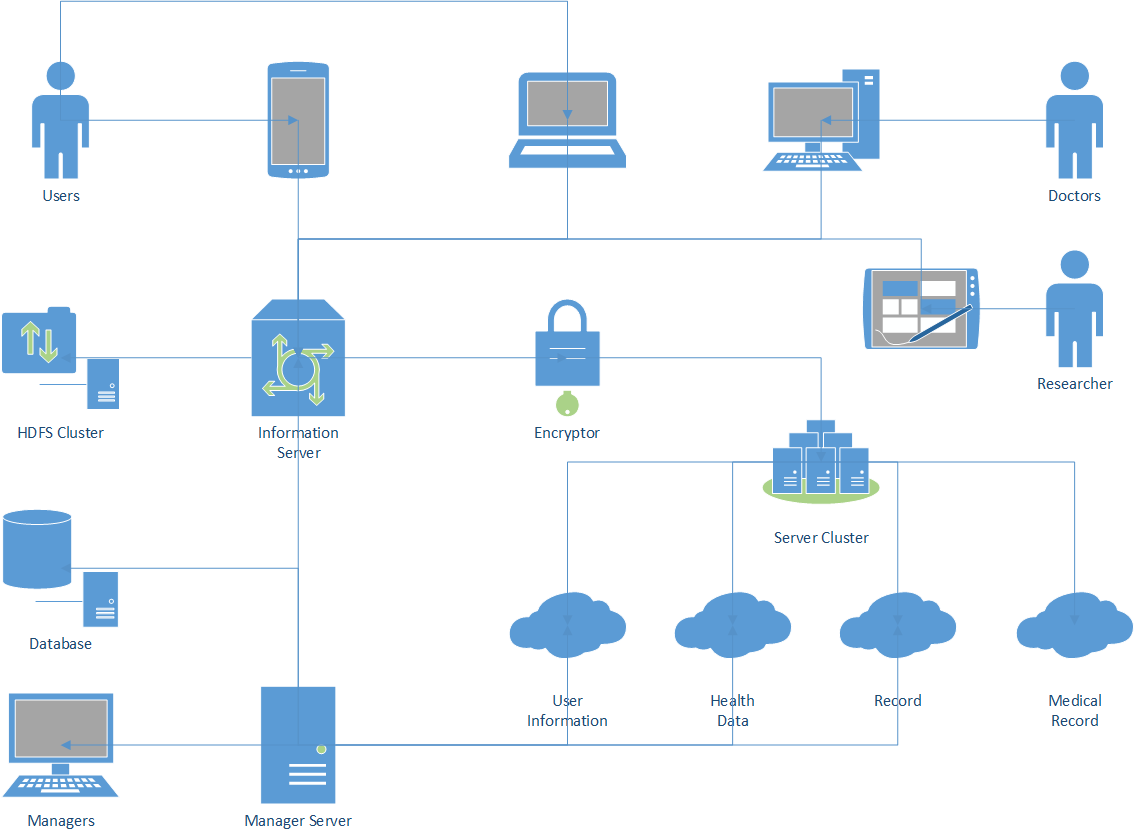
\includegraphics[width=14cm]{figures/arch.png}
    %     \caption{Architecture}
    % \end{figure} 

\end{document}
% \end{CJK}